\documentclass[11pt]{article}
\usepackage{amsmath, amsthm, amssymb, pdfpages} 
\usepackage{fullpage}
\usepackage{hyperref}
\usepackage{graphicx}
\usepackage[capitalize]{cleveref}

% next three for UTF8 to work (for non-ASCII names to work without awkward codes)
\usepackage[T1]{fontenc}
\usepackage{textcomp}
\usepackage[utf8]{inputenc}

% import biblatex with prefered settings
% reuse code and library from RGLS paper in the same repository
% loads biblatex with all the nice standard options that John determined some time ago!
% this version uses a ``Harvard'' style (first author last name, year in parentheses).
% also loads xpatch

% biblatex
% harvard style
\usepackage[style=authoryear,natbib,maxcitenames=2,doi=false,isbn=false,url=false,backend=bibtex]{biblatex}
% numeric style
%% \usepackage[style=numeric-comp,sorting=none,giveninits=true,
%%                      doi=false,isbn=false,url=false,backend=bibtex]{biblatex}
% remove "In: " before journal title
\renewbibmacro{in:}{}
% remove language
\AtEveryBibitem{\clearlist{language}}
% remove month
\AtEveryBibitem{\clearfield{month}}
% and also notes
\AtEveryBibitem{\clearfield{note}}
% remove dots between volume and issue
\usepackage{xpatch}
\xpatchbibmacro{volume+number+eid}{%
  \setunit*{\adddot}%
}{%
}{}{}
% put issue in parentheses
\DeclareFieldFormat[article]{number}{\mkbibparens{#1}}


\bibliography{../manuscripts/zotero, ../manuscripts/dummy} % biblatex wants this in the preamble...

% define shortcuts for awkward math symbols
% this also helps us change them more easily later, if needed
\newcommand{\rmsd}{\text{RMSD}_p}
\newcommand{\auc}{\text{AUC}_\text{PR}}

\usepackage[noT]{kinshipsymbols}
% % copy of \Fst from package `kinshipsymbols`
%\newcommand{\Fst}{F_\text{ST}}

% double line spacing (PLoS wants this)
\usepackage{setspace}
\doublespacing
% original, smaller spacing
%\renewcommand{\baselinestretch}{1.2}

\title{\Large \textbf{Testing the effectiveness of principal components in adjusting for relatedness in genetic association studies}}
\author{Yiqi Yao$^1$, Alejandro Ochoa$^{1,2,*}$}
\date{}

\begin{document}
\maketitle

\noindent
$^1$ Department of Biostatistics and Bioinformatics, Duke University, Durham, NC 27705, USA \\
$^2$ Duke Center for Statistical Genetics and Genomics, Duke University, Durham, NC 27705, USA \\
$^*$ Corresponding author: \texttt{alejandro.ochoa@duke.edu}


\begin{abstract}
  The genome-wide association study is widely used to identify the association between loci and trait.
  However, admixture population is involved in the current GWAS research which may result in the violation of Hardy-Weinberg Equilibrium (HWE).
  PCA can be used to correct for the bias result from admixture population.
  In this paper, we test the performance of PCA with desirable admixture simulation population.
  Since previous research about comparing PCA and LMM is limited, we also make comparison of performance among PCA, LMM and LM in terms of both power and type one error controlling.
  The approach we used in this paper is mainly based on the additive linear model.
  Since the number of loci we consider is much larger than sample size, each loci together with PCs is fitted to test the significance of this loci.
  According to the admixture simulation structure, three scenarios are considered in this case: large sample size, small sample size and large sample with complicated family structure.
  In these three scenarios, the number of loci and subpopulation are fixed.
  In order to fully compare the performance of PCA, LMM and LM under different admixture structures, Root mean square deviation (RMSD) and areas under curve (AUC) to measure the performance of type one error controlling and power separately.
  According to the results of simulation, it can be seen that PCA fails in both type one error and power when the number of PCA is smaller than the true rank of genotype matrix.
  Additionally, PCA is robust to type one error once the number of PCs is larger than true rank of genotype matrix regardless of sample size, but the existence of family structure will impose a negative influence on it.
  In terms of power, PCA will be punished with excessive usage of PCs in the case of small sample size.
  Once enough PCs are used in PCA, it always outperforms LM in both type one error controlling and power.
  Regarding LMM, it has similar performance to PCA in type one error controlling without complicated family structure, however, it has advantage over PCA when complex family structure exists.
  Considering power, LMM has better performance of power than PCA without complex family structure even enough PCs are used, whereas, the existence of complicated family structure will lead to PCA outperforms LMM in terms of power. 
\end{abstract}

\clearpage

\tableofcontents

\clearpage
	
\section{Introduction} 

The goal of a genome-wide association study (GWAS) is to identify loci whose genotypes are correlated significantly with a certain trait.
An important assumption made by basic association tests is that genotypes at non-associated loci are drawn independently from a common allele frequency, so that they are in Hardy-Weinberg Equilibrium (HWE).
However, HWE does not hold for structured populations, which includes multiethnic cohorts and admixed individuals, and for family data.
When naive approaches are incorrectly applied to structured populations and/or family data, association statistics (such as $\chi^2$) become inflated relative to the null expectation, resulting in greater numbers of false positives than expected \citep{devlin_genomic_1999, voight_confounding_2005, astle_population_2009}.

Modern approaches for conducting genetic association studies with structured populations involve modeling the population structure via covariates.
Such covariates may be inferred ancestry proportions \citep{pritchard_association_2000} or transformations of these.
Principal components analysis (PCA) represents the most common of these variants, in which the top eigenvectors of the kinship matrix are used to model the population structure \citep{price_principal_2006}.
These top eigenvectors are commonly referred to as Principal Components (PCs) in the genetics literature (the convention we adopt here; \cite{patterson_population_2006}), but it is worth noting that in other fields the PCs would instead denote the projections of the data onto the eigenvectors.
Various works have found that PCs map to ancestry, and PCs work as well as ancestry in GWAS and can be inferred more quickly \citep{patterson_population_2006}.

The other dominant approach for genetic association studies under population structure is the Linear Mixed-effect Model (LMM), in which population structure is a random effect drawn from a covariance model parametrized by the kinship matrix.
LMM and PCA share deep connections that suggest that both models ought to perform similarly \citep{hoffman_correcting_2013}.
However, many previous studies have found that LMM outperforms the PCA approach, although many evaluations are inconclusive or are limited to unrealistic population structures often with unrealistically low differentiation \citep{astle_population_2009, kang_variance_2010, price_new_2010, wang_analytical_2013}.
Moreover, various explanations for if and why LMM outperforms PCA are vague and have not been tested directly \citep{price_new_2010, sul_mixed_2013, price_response_2013}.
Since LMMs tend to be considerably slower than the PCA approach, it is important to understand when the difference in performance between these two approaches is outweighed by their difference in runtime.

In this work, we study the performance of the PCA method for GWAS, comparing it to a leading LMM approach, characterizing its behavior under various numbers of PCs and varying sample sizes, under a reasonable admixture model and a model with admixture and family structure.
Our evaluation is more thorough than previous ones, directly measuring the uniformity of null p-values (as required for accurate FDR control via q-values; \cite{storey_positive_2003, storey_statistical_2003}) and orthogonally measuring predictive power by calculating the area under precision-recall curves.
We find that the performance of the PCA approach is favorable when sample sizes are large (at least 1,000 individuals), matching the performance of LMMs as long as enough PCs are used.
Remarkably, the approach is robust even when the number of PCs far exceeds the optimal number, suggesting that the degrees of freedom is not a concern in reasonably large studies.
However, for smaller studies (100 individuals) there is a more pronounced loss of power when the number of PCs exceeds the optimal number.
Moreover, LMMs outperform PCA in the presence of family structure, which is a well-known scenario where the problematic structure is not low-dimensional so PCA naturally cannot model it entirely \citep{patterson_population_2006, price_new_2010}.
All together, our simulation studies provide clear criteria under which use of PCA results in acceptable performance compared to LMMs.

% TODO Missing:
% \begin{itemize}
% \item Proposed simulation to infer optimal number of PCs from real data, predict gap between PCA and LMM?
% \item LMM + 10 PCs approach
% \end{itemize}

\section{Methods}

\subsection{Models for genetic association studies}

In this subsection we describe the complex trait model and kinship model that motivates both the PCA and LMM models for genetic association studies, followed by further details regarding the PCA and LMM approaches.

\subsubsection{The additive quantitative trait model and PCA approximation}

Let $\xij \in \{ 0, 1, 2 \}$ be the genotype at locus $i$ for individual $j$, which counts the number of reference alleles.
Suppose there are $n$ individuals and $m$ loci,
$\mathbf{X} = ( \xij )$ is their $m \times n$ genotype matrix, and
$\mathbf{y}$ is the length-$n$ (column) vector which represents trait value for each individual.
The approaches we consider are based on the following additive linear model for a quantitative (continuous) trait:
\begin{equation}
  \label{eq:trait}
  \mathbf{y}
  =
  \mathbf{1} \alpha + \mathbf{X}^\intercal \mathbf{\beta} + \mathbf{\epsilon}
  ,
\end{equation}
where
$\mathbf{1}$ is a length-$n$ vector of ones,
$\alpha$ is the scalar intercept coefficient,
$\mathbf{\beta}$ is the length-$m$ vector of locus effect sizes, and
$\mathbf{\epsilon}$ is a length-$n$ vector of residuals.
The residuals are assumed to follow a normal distribution: $\mathbf{\epsilon}_j \sim \text{Normal}(0, \sigma^2)$ independently for each individual $j$, for some residual variance parameter $\sigma^2$.

Typically the number of loci $m$ is in the order of millions while the number of individuals $n$ is in the thousands.
Hence, the full model above cannot be fit in this typical $n \ll m$ case, as there are only $n$ datapoints to fit (the trait vector) but there are $m+1$ parameters to fit ($\alpha$ and the $\mathbf{\beta}$ vector).
The PCA model with $r$ PCs corresponds to the following approximation to the full model, corresponding to a model fit at a single locus $i$:
\begin{equation}
  \label{eq:pca_gwas}
  \mathbf{y}
  =
  \mathbf{1} \alpha + \mathbf{x}_i \beta_i + \mathbf{U}_r \mathbf{\gamma}_r + \mathbf{\epsilon}
  ,
\end{equation}
where $\mathbf{x}_i$ is the length-$n$ vector of genotypes at locus $i$ only,
$\beta_i$ is the effect size coefficient for that locus,
$\mathbf{U}_r$ is an $n \times r$ matrix of PCs, and
$\mathbf{\gamma}_r$ is the length-$r$ vector of coefficients for the PCs.
This approximation is explained by first noticing that the genotype matrix has the following singular value decomposition:
$\mathbf{X}^\intercal = \mathbf{U} \mathbf{D} \mathbf{V}^\intercal$,
where assuming $n < m$ we have that
$\mathbf{U}$ is an $n \times n$ matrix of the left singular vectors of $\mathbf{X}$,
$\mathbf{V}$ is an $m \times n$ matrix of its right singular vectors, and
$\mathbf{D}$ is an $n \times n$ diagonal matrix of its singular values.
Thus, in the full model we have
$\mathbf{X}^\intercal \mathbf{\beta} = \mathbf{U} \mathbf{\gamma}$,
where
$\mathbf{\gamma} = \mathbf{D} \mathbf{V}^\intercal \mathbf{\beta}$ is a length-$n$ vector.
The approximation consists solely of replacing $\mathbf{U} \mathbf{\gamma}$ (the full set of $n$ left singular vectors and their coefficients) with $\mathbf{U}_r \mathbf{\gamma}_r$ (the top $r$ singular vectors only, which constitutes the best approximation of rank $r$).
Thus, the extra terms in the PCA approach approximate the polygenic effect of the whole genome, and assumes that the locus $i$ being tested does not contribute greatly to this signal.

The statistical significance of a given association test is performed as follows.
The null hypothesis is $\beta_j = 0$ (no association).
The null and alternative models are each fit (fitting the coefficients of the multiple regression, where $\beta_j$ is excluded under the null while it is fit under the alternative).
The resulting regression residuals are compared to each other using the F-test, which results in a two-sided p-value.
Note that many common PCA implementations trade the more exact F-test for a $\chi^2$ test, which is simpler to implement but only asymptotically accurate.
As this is a multiple hypothesis test, there are a large number of loci ($m$) tested for association, so it is best to control the FDR rather than setting a fixed p-value threshold.
We recommend estimating q-values and setting a threshold of $q < 0.05$ so that the FDR is controlled at the 5\% level.

\subsubsection{Kinship model for genotypes}

In order to better motivate the most common estimation procedure of PCs for genotype data, and to connect PCA to LMMs, we shall review the kinship model for genotypes.
The model states that genotypes are random variables with a mean and covariance structure given by
$$
\E[ \xij ]
=
2 \pit,
\quad\quad
\Cov( \xij, \xij[k] )
=
4 \pit ( 1 - \pit ) \kt,
$$
where \pit is the ancestral allele frequency at locus $i$ and \kt is the kinship coefficient between individuals $j$ and $k$ \citep{malecot_mathematiques_1948, wright_genetical_1951, jacquard_structures_1970}.
Thus, if we standardize the genotype matrix as
$$
\mathbf{X}_S
=
\left(
  \frac{
    \xij - 2 \pit
  }{
    \sqrt{4 \pit \left( 1 - \pit \right)}
  }
\right)
,
$$
then this results in a straightforward kinship matrix estimator:
$$
\E
\left[
\frac{1}{m}
\mathbf{X}_S^\intercal
\mathbf{X}_S
\right]
=
\mathbf{\Phi}
,
$$
where $\mathbf{\Phi} = ( \kt )$ is the $n \times n$ kinship matrix.
Note that replacing the raw genotype matrix $\mathbf{X}$ with the standardized matrix $\mathbf{X}_S$ in the trait model of \cref{eq:trait} results in an equivalent model, as this covariate differs only by a linear transformation.
Thus, under the standardized genotype model, the PCs of interest are equal in expectation to the top eigenvectors of the kinship matrix.

\subsubsection{Estimation of principal components from genotype data}

In practice, the matrix of principal components $\mathbf{U}_r$ in \cref{eq:pca_gwas} is determined from an estimate of the earlier standardized genotype matrix $\mathbf{X}_S$, namely
$$
\mathbf{\hat{X}}_S
=
\left(
  \frac{
    \xij - 2 \pith
  }{
    \sqrt{4 \pith \left( 1 - \pith \right)}
  }
\right)
,
$$
where the true ancestral allele frequency \pit is replaced by the estimate
$
\pith = \frac{1}{2n} \sum_{j = 1}^n \xij,
$
and results in the kinship estimate
$
\mathbf{\hat{\Phi}}
=
\frac{1}{m}
\mathbf{\hat{X}}_S^\intercal
\mathbf{\hat{X}}_S
.
$
This kinship estimate and minor variants are also employed in LMMs \citep{yang_gcta:_2011}.
This estimator of the kinship matrix is biased, and this bias is different for every individual pair \citep{ochoa_fst2, ochoa_human}.
However, in the present context of PCA regression in genetic association studies, the existing approach performs as well as when the above estimate is replaced by the true kinship matrix (not shown).
Thus, it appears that in combination with the intercept term ($\mathbf{1} \alpha$ in \cref{eq:pca_gwas}), the rowspace of this kinship matrix estimate approximately equals that of the true kinship matrix.

\subsubsection{Linear mixed-effects model}

The LMM is another approximation to the complex trait model in \cref{eq:trait}, given by
\begin{equation}
  \label{eq:lmm_gwas}
  \mathbf{y}
  =
  \mathbf{1} \alpha + \mathbf{x}_i \beta_i + \mathbf{s} + \mathbf{\epsilon}
  ,
\end{equation}
which is like the PCA model in \cref{eq:pca_gwas} except that the PC terms $\mathbf{U}_r \mathbf{\gamma}_r$ are replaced by the random effect $\mathbf{s}$, which is a length-$n$ vector drawn from
$$
\mathbf{s} \sim \text{Normal} \left( \mathbf{0}, \sigma^2_s \mathbf{\Phi} \right),
$$
where $\mathbf{\Phi}$ is the kinship matrix and $\sigma^2_s$ is a trait-specific scaling factor.
This model is derived from treating the standardized genotype matrix $\mathbf{X}_S$ as random rather than fixed, so that the standardized genetic effect
$\mathbf{X}_S^\intercal \mathbf{\beta}_S$
in \cref{eq:trait} has mean zero and a covariance matrix of
$$
\Cov ( \mathbf{X}_S^\intercal \mathbf{\beta} )
=
|| \mathbf{\beta}_S ||^2 \mathbf{\Phi}
.
$$
The above random effect $\mathbf{s}$ satisfies those equations, where the variance scale equals $\sigma^2_s = || \mathbf{\beta}_S ||^2$.
Thus, the PCA approach is the fixed model equivalent of the LMM under the additional approximation that only the top $r$ eigenvectors are used in PCA whereas the LMM uses all eigenvectors.

A key advantage of LMM over PCA is that it has fewer degrees of freedom: ignoring the shared terms in \cref{eq:pca_gwas} and \cref{eq:lmm_gwas}, PCA has $r$ parameters to fit (each PC coefficient in the $\mathbf{\gamma}$ vector), whereas LMMs only fit one additional parameter, namely $\sigma^2_s$.
The difference is therefore expected to be more substantial when $r$ is very large and when the sample size (the number of individuals $n$) is very small.

Due to its accuracy and speed, the LMM implementation that we chose for our evaluations is GCTA \citep{yang_gcta:_2011}.

\subsection{Simulations}

\subsubsection{Genotype simulation from the admixture model}

We consider three simulation scenarios, refered to as (1) large sample size, (2) small sample size, and (3) family structure.
All cases are based on the admixture model described previously \citep{ochoa_fst1, ochoa_fst2}, and which is implemented in the R package \texttt{bnpsd} available on GitHub and the Comprehensive R Archive Network (CRAN).

Here we consider scenarios where the number of individuals $n$ varies:
the large sample size and family structure scenarios have $n = 1,000$ whereas small sample size has $n = 100$.
The number of loci in all cases is $m = 100,000$.
Individuals are admixed from $K = 10$ intermediate subpopulations, where $K$ is also the rank of the population structure; thus, after taking into account the intercept's rank-1 contribution, the population structure can be fit with $r = K-1$ PCs.
Each subpopulation $S_u$ ($u \in \{ 1, ..., K \}$) has an inbreeding coefficient $\ft[S_u] = u \tau$, individual-specific admixture proportions $q_{ju}$ for individual $j$ and intermediate subpopulation $S_u$ arise from a random walk model for the intermediate subpopulations on a 1-dimensional geography with spread $\sigma$, where the free parameters $\tau$ and $\sigma$ are fit to result in $\Fst = 0.1$ for the admixed individuals and a bias coefficient of $s = 0.5$, exactly as before \citep{ochoa_fst2}.

Random genotypes are drawn from this model, as follows.
First, uniform ancestral allele frequencies \pit are drawn.
The allele frequency $p_i^{S_u}$ at locus $i$ of each intermediate subpopulation $S_u$ is drawn from the Beta distribution with mean \pit and variance $\pit(1-\pit) \ft[S_u]$ \citep{balding_method_1995}.
The individual-specific allele frequency of individual $j$ and locus $i$ is given by
$
\pi_{ij} = \sum_{u = 1}^K q_{ju} p_i^{S_u}.
$
Lastly, genotypes are drawn from $\xij \sim \text{Binomial}(2, \pi_{ij})$.
Loci that are fixed (where for some $i$ we had $\xij = 0$ for all $j$, or $\xij = 2$ for all $j$) are drawn again from the model, starting from \pit, iterating until no loci are fixed.

\subsubsection{Genotype simulation from the family model}

Here we describe a simulation of a family structure with admixture that aims to be realistic by:
(1) pairing all individuals in every generation, resulting in two children per couple;
(2) strictly avoiding close relatives when pairing individuals;
(3) strongly favoring pairs that are nearby in their 1-dimensional geography, which helps preserve the population structure across the generations by preferentially pairing individuals with more similar admixture proportions (a form of assortative mating); and
(4) iterating for many generations so that a broad distribution of close and distant relatives is present in the data.

Generation 1 has individuals with genotypes drawn from the large sample size scenario described earlier, which features admixture.
In subsequent generations, every individual is paired as follows.
The local kinship matrix of individuals is stored and updated after every generation, which records the pedigree relatedness; in the first generation, everybody is locally unrelated.
Also, individuals are ordered, initially by the 1-dimensional geography, and in subsequent generations paired individuals are grouped and reordered by their average coordinate, preserving the original order when there are ties.
For every remaining unpaired individual, one is drawn randomly from the population, and it is paired with the nearest individual that is not a second cousin or closer relative (local kinship must be $< 1/4^3$).
Note that every individual is initially genderless, and after pairing one individual in the pair may be set to male and the other to female without giving rise to contradictions.
If there are individuals that could not be paired (occurs if unpaired individuals are all close relatives), then the process of pairing individuals randomly is repeated entirely for this generation.
If after 100 iterations no solution could be found randomly (there were always unpaired individuals), then the simulation restarts from the very first generation; this may occur for very small populations, but was not observed when $n = 1000$.
Once individuals are paired, two children per pair have their genotypes drawn independently of each other.
In particular, at every locus, one allele is drawn randomly from one of the parents and the other allele from the other parent.
Loci are constructed independently of the rest (no linkage disequilibrium).
The simulation continues for 20 generations.
As this simulation is very computationally expensive, it was run only once (genotypes did not change as new random traits were constructed as described next).

\subsubsection{Trait Simulation}

For a given genotype matrix (simulated or real), a simulated complex trait that follows the additive quantitative trait model in \cref{eq:trait} is constructed as follows.
In all cases we set the heritability of the trait to be $h^2 = 0.8$.
We varied the number of causal loci ($m_1$) together with the number of individuals ($n$) so power would remain balanced:
for the $n = 1,000$ cases we set $m_1 = 100$, whereas the $n = 100$ simulation had $m_1 = 10$.

Each simulation replicate consists of different causal loci with different effect sizes, as follows.
The non-genetic effects are drawn from $\epsilon_j \sim \text{Normal}(0, 1 - h^2 )$ independently for each individual $j$.
A subset of size $m_1$ of loci was selected at random from the genotype matrix to be causal loci.
The effect size $\beta_i$ at each causal locus $i$ is drawn initially from a Standard Normal distribution.
At non-causal loci $i$ we have $\beta_i = 0$.
Under the kinship model, the resulting genetic variance component is given by
$$
\sigma^2_0
=
\sum_{i = 1}^m 2 \pit ( 1 - \pit ) \beta_i^2 ,
$$
where \pit is the true ancestral allele frequency at locus $i$, which is known in our simulations.
The desired genetic variance of $h^2$ is therefore obtained by multiplying every $\beta_i$ by $\frac{h}{ \sigma_0 }$.
Lastly, the intercept coefficient in \cref{eq:trait} is set to $\alpha = - \sum_{i=1}^m 2 \pit \beta_i$, so the trait expectation is zero.
This trait simulation procedure is implemented in the \texttt{simtrait} R package, available at
\url{https://github.com/OchoaLab/simtrait}.

\subsection{Evaluation of performance}

All of the approaches considered here are evaluated in two orthogonal dimensions.
The first one---the $\rmsd$ statistic below---quantifies the extent to which null p-values are uniform, which is a prerequisite for accurate control of the type-I error and successful FDR control via q-values.
The second measure---the area under the precision-recall curve---quantifies the predictive power of each method, which makes it possible to qualitatively compare the statistical power of each method without having to select a single threshold, and most importantly, overcoming the problem that methods may not have accurate p-values.

\subsubsection{$\rmsd$: a measure of p-value uniformity}

From their definition, correct p-values (for continuous test statistics) have a uniform distribution when the null hypothesis holds.
This fact is crucial for accurate control of the type-I error, and is a prerequisite for the most common approaches that control the FDR, such as q-values \citep{storey_positive_2003, storey_statistical_2003}.
We use the Root Mean Square Deviation (RMSD) to measure the disagreement between the observed p-value quantiles and the expected uniform quantiles:
$$
\rmsd
=
\sqrt{ \frac{1}{m_0} \sum_{i = 1}^{m_0} \left( u_i - p_{(i)} \right)^2 },
$$
where
$m_0 = m - m_1$ is the number of null loci ($\beta_i = 0$ cases only),
here $i$ indexes null loci only,
$p_{(i)}$ is the $i$th ordered null p-value, and
$u_i = ( i - 0.5 ) / m_0$ is its expectation.
Thus, $\rmsd = 0$ corresponds to the best performance in this test, and larger $\rmsd$ values correspond to worse performance.

In previous evaluations, test statistic inflation has been used to measure the success of corrections for population structure \citep{astle_population_2009, price_new_2010}.
The inflation factor $\lambda$ is defined as the median $\chi^2$ association statistic divided by theoretical median under the null hypothesis \citep{devlin_genomic_1999}.
Hence, when null test statistics have their expected distribution, we get $\lambda = 1$ (same as $\rmsd = 0$ above).
However, any other null test statistic distribution with the same median results in $\lambda = 1$ as well, which is a flaw of this test that $\rmsd$ overcomes ($\rmsd = 0$ if and only if null test statistics have their expected distribution).
The $\lambda > 1$ case (gives $\rmsd > 0$) corresponds to inflated statistics, which occurs when residual population structure is present.
$\lambda < 1$ is not expected for genetic association studies (also gives $\rmsd > 0$).
Note that $\lambda$ only use the median of the null distribution, whereas the $\rmsd$ makes use of the complete p-value distribution to evaluate its uniformity, which is more accurate.

\subsubsection{The area under the precision-recall curve}

Precision and recall are two common measures for evaluating binary classifiers.
Let $c_i$ be the the true classification of locus $i$, where $c_i = 1$ for truly causal loci (if the true $\beta_i \ne 0$, where the alternative hypothesis holds), and $c_i = 0$ otherwise (null cases).
For a given method and some threshold $t$ on its per-locus test statistics, the method predicts a classification $\hat{c}_i(t)$ (for example, if $t_i$ is the test statistic, the prediction could be $\hat{c}_i(t) = 1$ if $t_i \ge t$, and $\hat{c}_i(t) = 0$ otherwise).
Across all loci, the number of true positives (TP), false positives (FP) and false negatives (FN) at the given threshold $t$ is given by
\begin{align*}
  \text{TP}(t)
  &=
    \sum_{i = 1}^m c_i \hat{c}_i(t)
    , \\
  \text{FP}(t)
  &=
    \sum_{i = 1}^m (1 - c_i) \hat{c}_i(t)
    , \\
  \text{FN}(t)
  &=
    \sum_{i = 1}^m c_i \left( 1 - \hat{c}_i(t) \right)
    .
\end{align*}
Precision and recall at this threshold are given by
\begin{align*}
  \text{Precision}(t)
  &=
    \frac{ \text{TP}(t) }{ \text{TP}(t) + \text{FP}(t) }
    =
    \frac{ \sum_{i = 1}^m c_i \hat{c}_i(t) }{ \sum_{i = 1}^m \hat{c}_i(t) }
    , \\
  \text{Recall}(t)
  &=
    \frac{ \text{TP}(t) }{ \text{TP}(t) + \text{FN}(t) }
    =
    \frac{ \sum_{i = 1}^m c_i \hat{c}_i(t) }{ \sum_{i = 1}^m c_i }
    .
\end{align*}
The precision-recall curve results from calculating the above two values at every threshold $t$, tracing a curve as recall goes from zero (everything is classified as null) to one (everything is classified as alternative), and the area under this curve is our final measure $\auc$.
A method obtains the maximum $\auc = 1$ if there is some threshold that classifies all loci perfectly.
In contrast, a method that classifies at random (for example, $\hat{c}_i(t) \sim \text{Bernoulli}(p)$ for any $p$) has an expected precision ($= \auc$) approximately equal to the overall proportion of alternative cases:
$\pi_1 = \frac{m_1}{m} = \frac{1}{m} \sum_{i = 1}^m c_i$.
The $\auc$ was calculated using the R package \texttt{PRROC}, which computes the area by integrating the correct non-linear piecewise function when interpolating between points \citep{grau_prroc:_2015}.



\section{Result}

We use simulation data where genotypes and trait will be simulated following procedure mentioned above.
We first set the sample size to be 1000 and then, we reduce the sample size to 100 to investigate whether PCA still have similar performance under new scenario.
We will conduct 10 times simulation so that the extra variance can be reduced.
For each simulation, performance of PCA will be collected in terms of RMSD and AUC for PCs from 2 to 90.
Also, real data set will also be introduced to test the performance of PCA and trait will be simulated in the same way to simulation data.
Then, we will test the performance of PCA when family structure exists with sample size equals to 1000 and 100 separately.
Finally, we test the performance of PCA with the existence of complex family structure and here we set the generation to be 20.

\subsection{PCA performance under N=1000}
\begin{figure}[bp!]
  \centering
  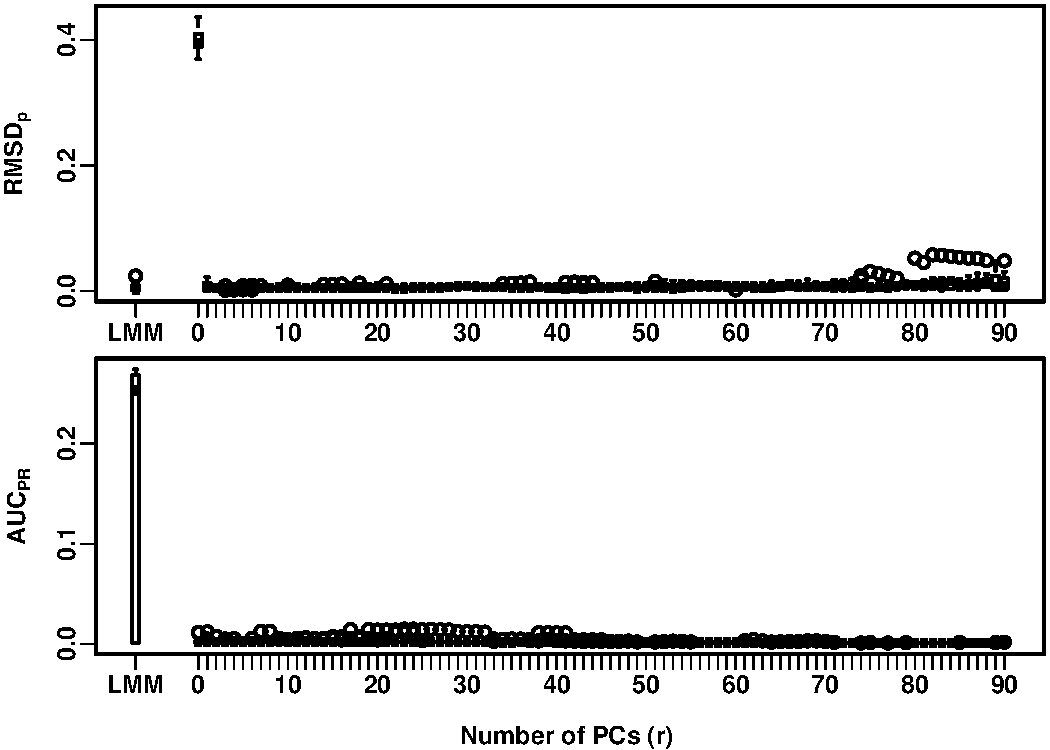
\includegraphics[width=4in]{PCA_n_1000_m_10_k_10.pdf}
  \caption{
    {\bf boxplot of rmsd and auc}
    The first panel is the boxplot of RMSD when sample size is 1000. Here the y axis represents value of rmsd and x axis is the number of PCs used in PCA.
    The second panel is the boxplot of AUC and here y axis is value of AUC. RMSD is used to measure the deviation of distribution of p values of null hypothesis from uniform distribution. In the case of multiple null hypothesis holds, the distribution of p-values of null hypothesis should approximate to unifrom distribution. The small value of RMSD implies type one error is well controlled. Regaring AUC, it's calculated by integration of predicion and recall curve. The value of AUC can be interpreted as the proportion of predictions made by this model is correct. The large AUC value implies better performance in predictive power. The result of Linear Regression is put at the position of PC equals to zero and the result of LMM is put at the position of PC equals to 91.}
  \label{fig:large_sample_size}
\end{figure}

According to \cref{fig:large_sample_size}A which is the boxplot of RSMD when the number of subpopulation is 10 and sample size is 1000, it can be seen that RMSD values remain relatively high when p is smaller than 9, which satisfies the actual rank of genotype matrix or kinship matrix which is (k-1).
It demonstrates that the distribution of p-values of null hypothesis deviates from the expected quantiles of uniform distribution and therefore, PCA fails to control FDR.
Though the performance of PCA is relatively bad, there still exists an decreasing tendency.
It indicates that when the number of PCs used in PCA is smaller than true rank of genotype matrix, PCA will benefit forom using more PCs in terms of controlling FDR.
However, once the number of PCs used in PCA reaches the actual rank of genotype matrix or kinship matrix, the RSDM will junmp to a small value and in this case the value of RMSD is close to 0.
It remains stable as the number of PCA increases.
Apart from this, it can be seen that before the number of PCs reaches the rank of genotype matrix, the distance among minimum and maximun of RMSD is larger.
It tends to be smaller after number of PCs used in PCA is larger than the rank of genotype matrix, which shows less fluctuations in terms of type 1 error controlling.
The RMSD value of LM is around 0.13 and it is smaller than PCA's RMSD value when PCs used in PCA is smaller than true rank of genotype matrix.
However, once the number of PCs is larger than true rank of genotype matrix, it can be seen that PCA has better performance in type one error controlling.
Compared with the performance of LMM, it can be seen that both PCA and LMM controll type one error well once the number of PCs used in PCA is larger than the true rank of genotype.

\cref{fig:large_sample_size}B illustrates the pattern of AUC for the same scenario to the first panel.
In this case, we can see a increasing tendency for AUC when the number of PCs is samller than the true rank of genotype or kinship matrix.
Such a tendency indicates that the increase of number of PCs can increase predictive power of PCA when it is smaller than the rank of genotype matrix.
Once the number of PCs used in PCA exceeds the rank of PCA, the value of AUC will be increased to around 0.8, which indicates that $80\%$ predictions of PCA are correct.
After that, PCA does not benefit from adding more PCs as it can not increase the value of AUC obviously.
Similarly, the range of AUC tends to be smaller than it when the number of PCs used in PCA is greater than rank of genotype matrix.
It is clear that LM has better performance when
Similar to the previous pandel, PCA outperforms LM when the number of PCs is no smaller than the true rank of genotype matrix.
In terms of LMM, the average AUC value is slightly higher than AUC of PCA even the number of PCs is larger than true rank of genotype matrix. 


\subsection{PCA performance under N=100}
\begin{figure}[bp!]
  \centering
  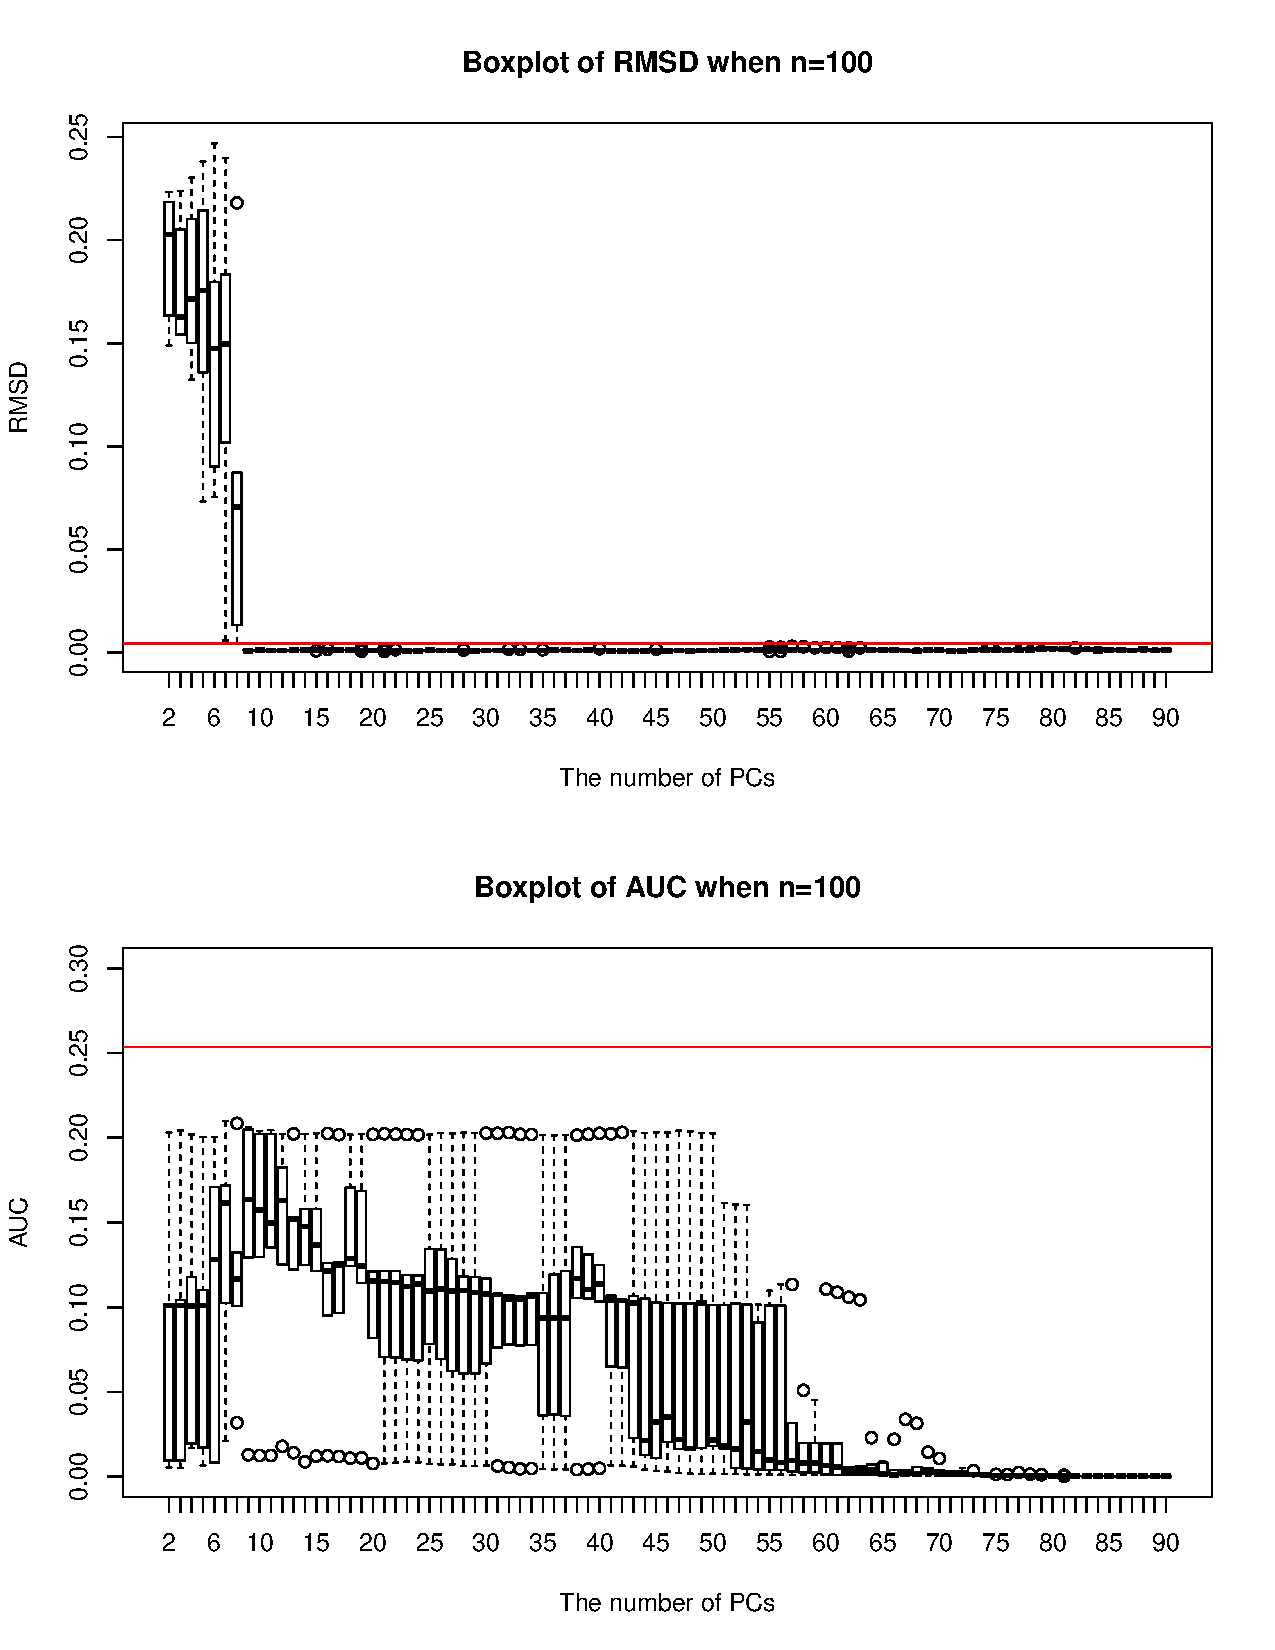
\includegraphics[width=4in]{PCA_n_100_m_10_k_10.pdf}
  \caption{
    {\bf boxplot of rmsd and auc}
    The first panel is the boxplot of RMSD when sample size is 100.
    The pattern of panel A in here is similar to \cref{fig:large_sample_size}A.
    The converging value of RMSD here is also close to zero indicating that even in a small sample size, PCA is still robust to type one error controlling.
    Moreover, the LMM and PCA has similar RSMD values which demonstrates that these two methods have almost the same performance in type one error controlling.
    The pattern of \cref{fig:large_sample_size}B is bell-shapled.
    The AUC value reaches the peak when the number of PCs used in PCA equals to 9 and begins to decrease with the increase of PCs used.
    It illustrates that PCA fails in terms of power when the sample size is small.
    The decrease tendency is more obvious when the number of PCs is around 68 and it can be seen that LMM which is located at the last point of y-axis has better performance in power, compared with PCA and LM.
  }
  \label{fig:small_sample_size}
\end{figure}

Then, we want to investigate the performance of PCA when samlpe size is small.
Here we set the sample size to be 100.
From \cref{fig:small_sample_size}A it can be seen that the pattern is similar to the boxplot of RMSD in the case of sample size equals to 1000.
It illustrates an decreasing when the number of PCs is smaller than true rank of genotype matrix.
It indicates that PCA can better control type 1 error in this situation.
If the number of PCs is greater than true rank of genotype matrix, the RSMD will decrease immediately and approximate to zero, which shows type one error is excellently controlled.
Hence, PCA is insensitive to the smaple size in terms of RMSD or type 1 error controlling.
Compared with the RMSD value of LM, RMSD value of PCA is smaller when the number of PCs is greater than 3.
It implies that PCA control type one error better than LM.
Moreover,the performance of LMM in this case is similar to \cref{fig:small_sample_size} which is close to previous figure.
The RMSD value of LMM approximates to 0 which indicates that there is no significant difference among PCA and LMM in this case.

\cref{fig:small_sample_size}B concerned with the boxplot of AUC, the pattern is obviously different from the boxplot of AUC when smaple size is 1000.
Although we still can find an increasing pattern of AUC before the number of PCs reaches the k.
However, it can be seen that there is an decreasing pattern of AUC value once the number of PCs exceeds the true rank of PCA.
It demonstrates that, even though fluctuations exist, performance of PCA in terms of power can be wrose with the increase of PCs used in PCA.
The position of peak of AUC in this case is located at PCs equal to 9 which is exactly the true rank of genotype.
Since we take the intercept into consideration, the true rank of genotype matrix equals to the number of subpopulation minus one.
The bell-shaled distribution of AUC boxpolot implies that PCA receives punishment in power once the number of PCs used in PCA is larger than true rank of genotype matrix.
Moreover, in terms of LM, it can be seen that even only one PC is used in PCA, the AUC value of PCA is still no worse than LM.
However, when excessive PCs are used, performance of LMM can be better with a larger AUC value.
Considering LMM, the average` AUC value is 0.25, whereas, the maximum AUC of PCA is 0.2 and it decreases immediately due to the excessive use of PCs.
In this case, LMM performs better than PCA in terms of power. 




\begin{figure}[bp!]
  \centering
  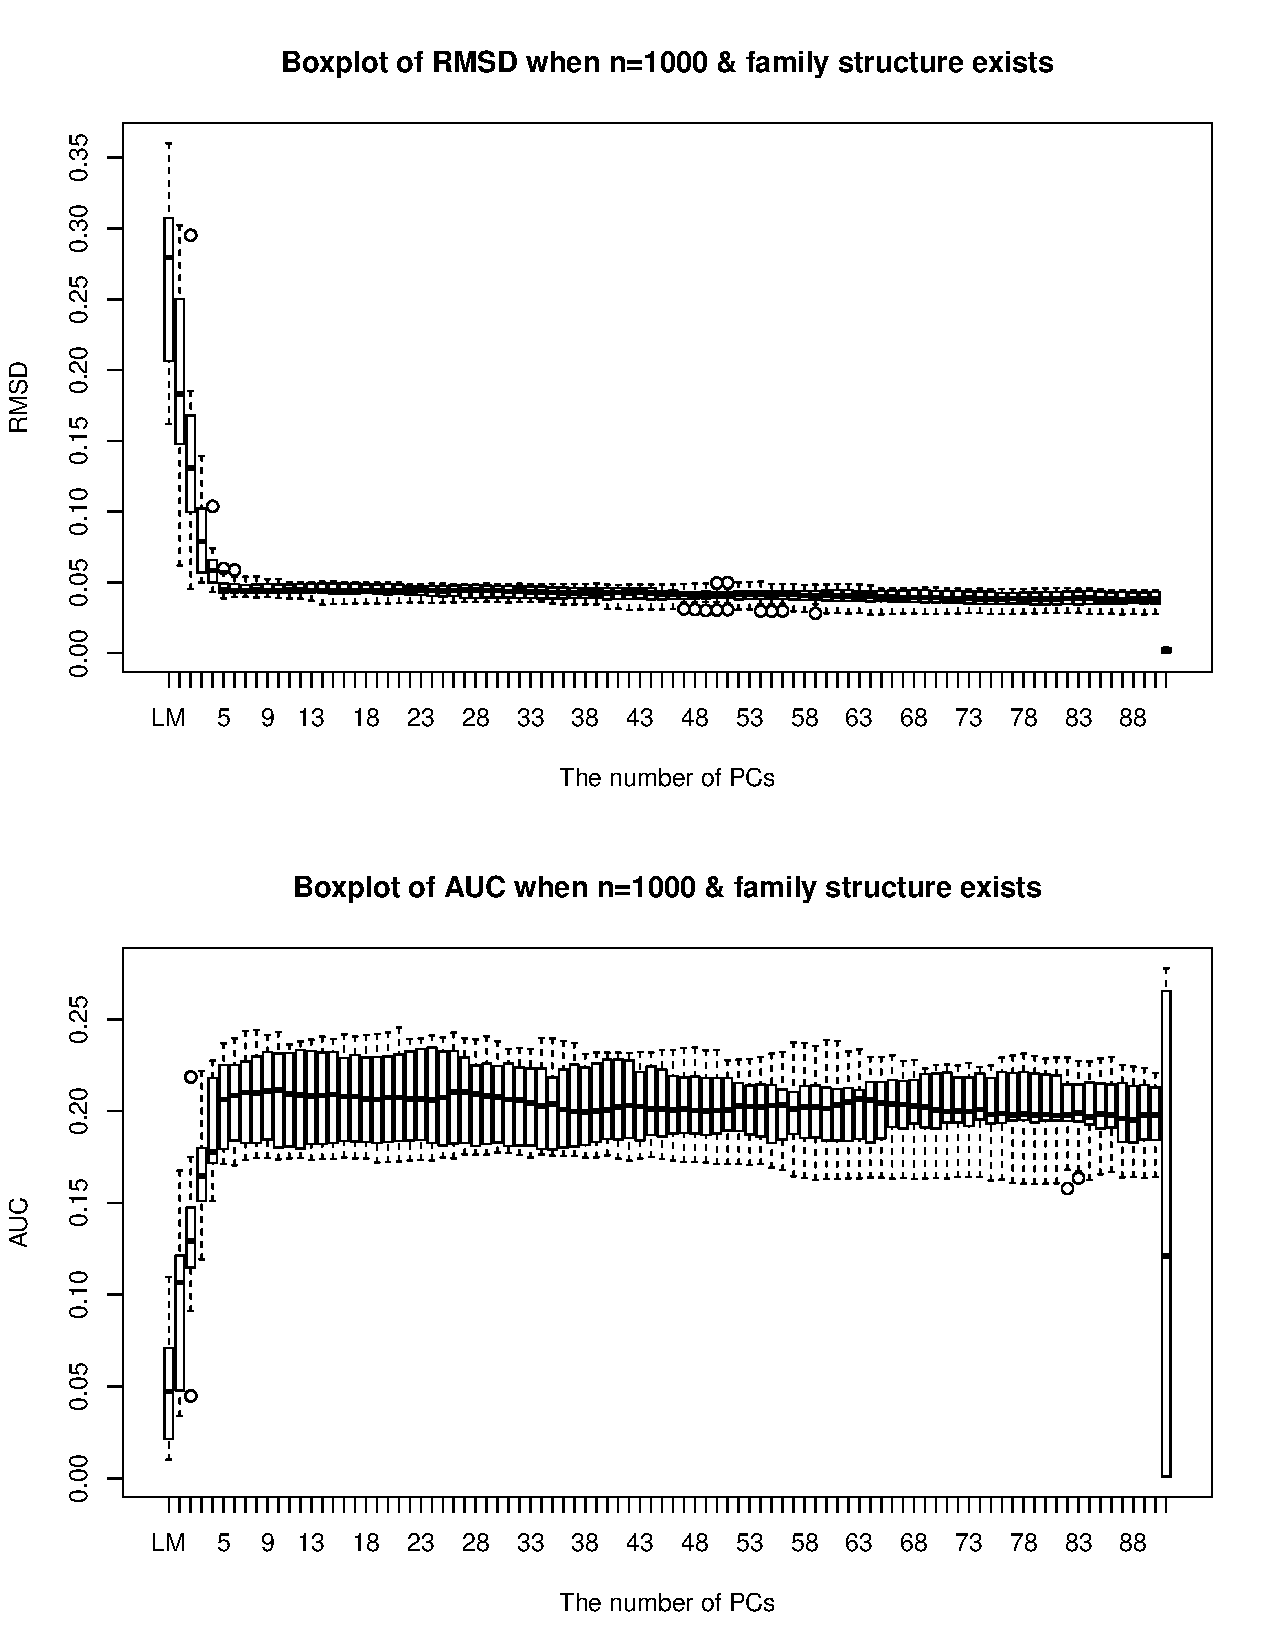
\includegraphics[width=4in]{PCA_n_1000_m_100_family_structure.pdf}
  \caption{
    {\bf boxplot of rmsd and auc}
    The first panel is the boxplot of RMSD when sample size is 100.
    The pattern of panel A here is similar to \cref{fig:large_sample_size}A.
    The converging value of RMSD here is also close to one indicating that even in a small sample size, PCA is still robust to type one error controlling.
    The pattern of panel B is bell-shapled.
    The AUC value reaches the peak when the number of PCs used in PCA equals to 9 and begins to decrease with the increase of PCs used.
    It illustrates that PCA fails in terms of power when the sample size is small.
  }
  \label{fig:family_structure}
\end{figure}

\subsection{PCA performance when familty structure exists}

The introduction of family structure will make the original admixture populatio more complicated.
In this case, we assume that there are 20 generations in total while other factors fixed.
Based on the result of \cref{fig:family_structure}A indicates that there is a decreasing pattern of RMSD for the first three PCs.
It addition, the value of RMSD in this situation is large, which indicates that the distribution of p-value of null hypothesis does not approximate to uniform distribution.
It illustrates that PCA fails to control type one error when the number of PCs is not enough.
When the number of PCs is larger than 4, values of RMSD beome stable around 0.05 which demonstrates that there exists evidence of the distribution of p-value of null hypothesis does not deviate from uniform distribution but the evidence is weaker than previous simulation where RSDM approximates to 0.
Considering the range of RMSD, it decreases first and then begins to increase.
It shows that excessive use of PCs will lead to extra variance.
In terms of LM, it can be seen that its RMSD value is around 0.28, which indicates that the distribution of p-value of null hypothesis is significantly deviated from uniform distribution. Hence, LM fails in the case of complicated family strcuture exists.  
For LMM, the value of RMSD still close to zero illustrating that type one error can be excellently controlled even when complicated family strcuture exists.
For AUC, it illustrates an increasing tendency for the first three PCs (\cref{fig:family_structure}B).
When the number of PCs is larger than 3, AUC fluctuates around 0.2.
This shows the power of PCA is small and hence, PCA's performance is not pretty well in this csae in terms of power even though enough PCs are used. 
Regarding LM, the value of AUC is smaller than PCA with 1 PC used. 
It shows that PCA outperforms LM in this case.
Considering LMM, the AUC value of PCA is larger than LMM when enough PCs are used in PCA and the range of AUC value of LMM is large.
Hence, PCA also outperforms LMM in terms of power.



\section{Discussion}

%\subsection{PCA GWAS fails without enough PCs}

Right now, both LMM and PCA have become standard approaches to correct for admixture population. In current PCA GWAS research, the number of PCs used in PCA is ususally assmued to be 10.
For instance, based on the simulation of \citet{hoffman_correcting_2013}, 10 PCs are randomly selected from the first 30 PCs.
Furthermore, \citet{wojcik_genetic_2019} also performed PCA GWAS for 26 traits with first 10 PCs.
According to the result of \citet{wojcik_genetic_2019}, the correlation plot between SNP genotype and PC1–PC10 illustrates different populations has different correlations over some PCs.
It seems that there exists a tradition that when PCA GWAS is performed, the top 10 PCs will be used.
Since the result of PCA GWAS in this convention is good, right now most paprs will assume the number of PCs used in PCA GWAS to be 10.
However, in this paper, we further investigate about the optimal choice of number of PCA under different population structures.
In most current research, the number of subpopulation is smaller 10 and thus, based on results of previous three scenarios, the number of PCs used in PCA is enough which certifies the good performance of PCA  in current research.
For instance, based on the scatter plot of first two principal components with HapMap3 dataset which contains 11 populations, it can be divided into three subpopulations (Gad and Machiel, 2014).
On the contraty, the lack of PCs will lead to the failure of PCA regardless of the sample size or family structure in both type one error and power.
Seokho et al.(2012) state that considering the large number of single-nucleotide polymorphisms (SNP) used in GWAS to infer structure, it is necessary to remove SNPs that have negligible loadings in PCA.
Whereas, our simulation indicates that if there is no enough PCs used in PCA GWAS, its performance can be bad as SNPs that have significant loadings are vanished from the analysis.

%\subsection{PCA GWAS still works even too many PCs are used}

PCA GWAS is still robust even though PCs are excessively used for type one error controlling. However, for power, it will receive punishment if the number of PCs are excessive and the sample size is small.
Jason and Anna (2009) point out that PCA with large sample size has better sample size than it with small sample size.
This is because that PCA with large sample size can have smaller probability error and larger accuracy of population estimation ( Jason and Anna ,2009).
The small sample size in our research project only has 100 individuals in total.
In a GWAS study, this is an extreme situation which it not realistic in research.
The AUC boxplot of small sample size indicates that the peak of AUC is close to AUC value for large sample size.
This may result from that the number of causal loci in small sample size is reduced from 100 to 10.
However, the boxplot of AUC has a bell shap with downward-sloping line on each side of the peak.
It demonstrates that in small sample size, punishment of excessive use of PCs will come occur immdeiately.
Considering in the study of GWAS, we will expect to use thousnds of SNPs and number of individuals are also much larger than 100, the situation of small sample size may not be common (Seokho et al., 2012).
Hence, although PCA will fail when the number of PCs is much larger than the true rank of genotype matrix, it is still encouraged to use more PCs in PCA GWAS.

%\subsection{PCA GWAS fails with the existence of complex family strcuture}

\citep{price_new_2010} point out that GWAS may fail in the case of dataset contains  family structure.
The result of our simulation also supports this argument.
\cref{fig:family_structure} shows that PCA has worse performance in type one error controlling when family strcuture exists, compared with \cref{fig:large_sample_size}.
Without complicated family structure, the vlaue of RMSD will converges to 0 when the number of PCs is large enough.
However, in the case of complex family structure, it can be seen that RMSD converges to 0.05 which indicates that we do not have strong evidence to claim that type one error is excellently controlled.
Concerning power, it can be seen that in both siutations, AUC will converge to 0.2.
Whereas, the range of AUC in \cref{fig:family_structure} will increase when excessive PCs are used in PCA.
It illustrates that excessive use of PCs will result in the extra variance. 
Hence, in the case of complex family structure, we need to be cautious about using PCs to aviod unnecessary variance. 

%\subsection{LMM outperforms PCA}

\citet{wang_analytical_2013} argues that mixed effects model is preferred in the case of existence cryptic relatedness but not population stratification.
In their paper, only first four PCs are used in PCA and performance of PCA may be underestimated.
Fruthermore, EMMAX which is a kind of linear mixed model is claimed to be better than PCA (Gengxin and Hongjiang, 2013).
Based on the result of our simulations, it can be seen that in both large sample size and small sample size, LMM are slightly better than PCA in terms of power.
When sample size is large such as the scenario in \cref{fig:large_sample_size}B, it can be seen that although both two methods's are not good.
However, the maximum AUC value of PCA is around 0.25 and LMM's AUC value is slightly larger than PCA.
In addition to this, in the case of small smaple size, advantage of LMM is more obvious.
As mentioned before, PCA will receive punishment when the number of PCs is much larger than the true rank of genotype matrix.
The maximum of AUC value of PCA in this scenario decreases to 0.2 and the average AUC value of LMM is around 0.24.
However, when complicated family structure exists, PCA outperforms LMM in terms of power. 

\citep{tucker_improving_2014}

TODO:
Gengxin and Hongjiang (2013) demonstrate that efficient mixed-model association eXpedited (EMMAX) which is based on linear mixed model outperforms PCA in both the population cohort study and case-control study.


\printbibliography



\end{document}